%!TEX root = Slic3r-Manual.tex

\section{Infill Optimization} % (fold)
\label{sec:infill_optimization}
\index{infill}

Slic3r contains several advanced infill settings which can help produce better extrusions.

\begin{figure}[H]
\centering
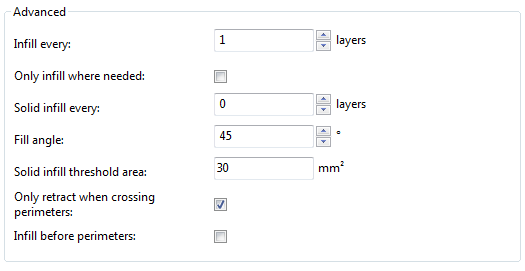
\includegraphics[keepaspectratio=true,width=1.0\textwidth]{expertmode/infill_advanced_settings.png}
\caption{Infill advanced settings.}
\label{fig:infill_settings}
\end{figure}

\begin{itemize}
    \item \texttt{Infill every \textit{n} layers} - Will produce sparse vertical infill by skipping a set number of layers. This can be used to speed up print times where the missing infill is acceptable.
    \item \texttt{Only infill where needed} - Slic3r will analyse the model and choose where infill is required in order to support internal ceilings and overhangs.  Useful for reducing time and materials.
    \item \texttt{Solid infill every \textit{n} layers} - Forces a solid fill pattern on the specified layers.  Zero will disable this option.
    \item \texttt{Fill angle} - By default the infill pattern runs at 45° to the model to provide the best adhesion to wall structures.  Infill extrusions that run adjacent to perimeters are liable to de-laminate under stress.  Some models may benefit from rotating the fill angle to ensure the optimal direction of the extrusion.
    \item \texttt{Solid infill threshold area} - Small areas within the model are usually best off being filled completely to provide structural integrity.  This will however take more time and material, and can result in parts being unnecessarily solid.  Adjust this option to balance these needs.
    \item \texttt{Only retract when crossing perimeters} - Retracting, to prevent ooze, is unnecessary if the extruder remains within the boundaries of the model.  Care should be taken if the print material oozes excessively, as not retracting may result in enough material loss to affect the quality of the subsequent extrusion.  However, most modern printers and materials rarely suffer from such extreme ooze problems.
    \item \texttt{Infill before perimeters} - Reverses the order in which the layer is printed. Usually the perimeter is laid down initially, followed by the infill, and this is usually the preferable as the perimeter acts as a wall containing the infill.
\end{itemize}


% section infill_optimization (end)